% 33-35(33쪽) — 35번 그림 · y=f(x) 의 그래프(x축을 점근선으로 오른쪽으로 갈수록 가파르게 커지는 곡선 · x=3 안내 점선). 스캔 화질이 낮아 TikZ 로 다시 그림.
% 원문에 있는 것만: x축 눈금 -2, 3 · y축 옆 1 · 점선 한 줄 · 라벨 y=f(x), O, x, y.
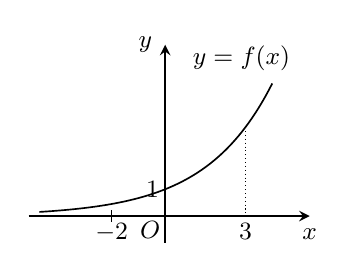
\begin{tikzpicture}[x=0.34cm, y=0.34cm, line width=0.6pt]
  \draw[->, >=stealth, line width=0.7pt] (-5.1,0) -- (5.4,0) node[below=1pt, font=\small] {$x$};
  \draw[->, >=stealth, line width=0.7pt] (0,-1.0) -- (0,6.4) node[left=1pt, font=\small] {$y$};
  \draw[densely dotted, line width=0.4pt] (3,3.32) -- (3,0);
  \draw[line width=0.6pt, domain=-4.7:4.0, samples=100, smooth] plot (\x, {exp(0.4*\x)});
  \draw[line width=0.5pt] (-2,-0.22) -- (-2,0.22);
  \node[font=\small, inner sep=2.5pt, below] at (-2,0) {$-2$};
  \node[font=\small, inner sep=2.5pt, below] at (3,0) {$3$};
  \node[font=\small, inner sep=1.5pt, below left] at (0,0) {$\pt{O}$};
  \node[font=\small, inner sep=2pt, left] at (0,1) {$1$};
  \node[font=\small, anchor=west, inner sep=1pt] at (0.9,5.9) {$y=f(x)$};
\end{tikzpicture}
